% pdflatex -shell-escape -interaction=nonstopmode main.tex && pdflatex -shell-escape -interaction=nonstopmode main.tex

\chapter{Definitionen}

% \begin{itemize}
%     \item Einführung in ML Algorithmen
%     \item ``Im folgenden werden wir ein paar Möglichkeiten in Betracht ziehen wie man Genetische Algorithmen für Black Box Optimierung benutzen kann''
%    \item ``Ausserdem verknüpfen wir diese mit einer Reduzierung vom Suchraum durch Fouriertransformationen und verwenden verschiedene Kodierung der Individuen, durch Normalverteilungen und direkt durch Zahlen''
% \end{itemize}

Dieses Kapitel bietet Einblick in die Grundlagen von \textbf{Genetischen Algorithmen} im Zusammenhang mit \textbf{neuronalen Netzen} und der \textbf{Cross Entropy Method}. Außerdem werden einige Verbesserungen zu den naiven Methoden besprochen, wie die Reduzierung des Suchraums durch \textbf{Fouriertransformationen} und die Einführung von einer \textbf{kooperativen Evolution} durch Hinzufügen von einer neuen Methode zum GA.

    \section{Genetische Algorithmen}
        % ``Die Motivation von Genetischen Algorithmen kam aus der Natur bla blubb''\\
        % ``Im Folgenden behandeln wir die grundlegenden Operationen die einen GA ausmachen''

        % Ein Genetischer Algorithmus gehört zu den \textbf{unsupervised Learning} Methoden, die sich als Ziel setzen eine verborgene Struktur zu analysieren, ohne zu gekenntzeichnete Daten zu haben. John Holland

        Ein genetischer Algorithmus ist ein Optimierungsverfahren, der meiner Meinung nach an einem natürlichen Vorgang am Besten zu erklären ist. Wir stellen uns beispielsweise zehn Antilopen und ein Gepard vor

        \begin{figure}[htbp]
            \begin{subfigure}{0.5\textwidth}
                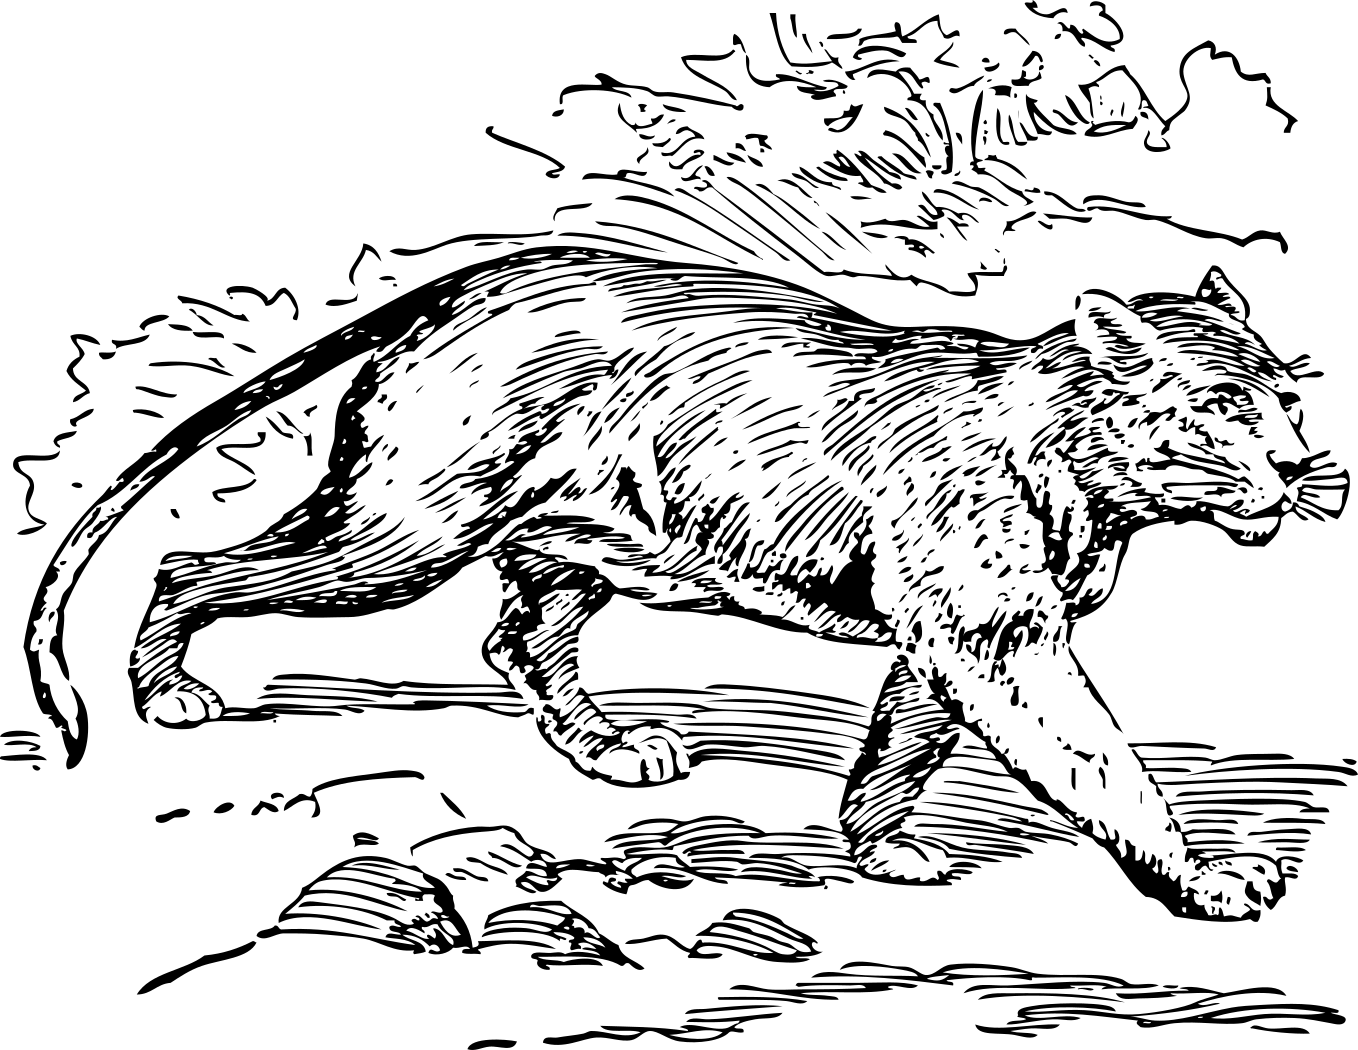
\includegraphics[width = 1\textwidth, left]{../pictures/cheetah.png}
            \end{subfigure}
            \begin{subfigure}{0.5\textwidth}
                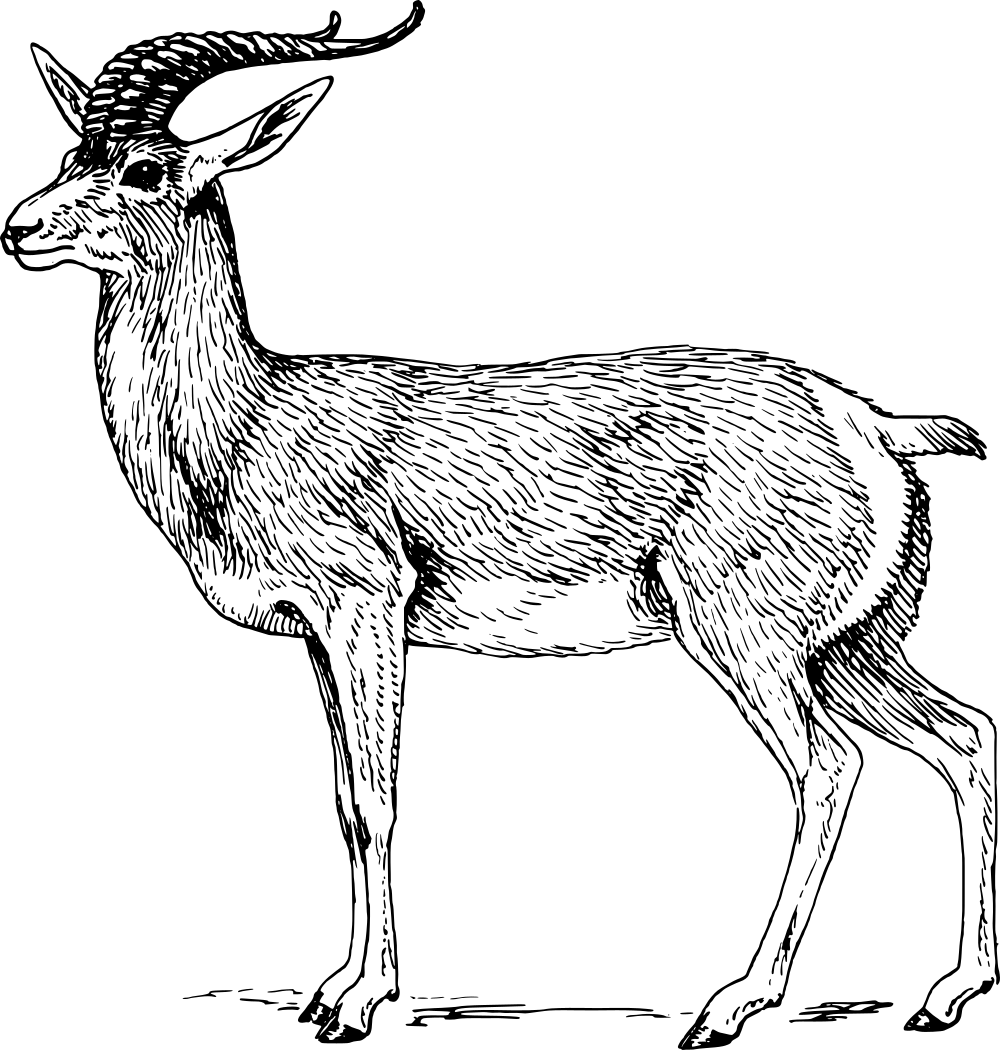
\includegraphics[width = 0.73\textwidth, right]{../pictures/antelope.png}
            \end{subfigure}
            \caption{Illustration von einem Geparden und einer Antilope \label{fig:somelabel}}
        \end{figure}





        \subsection{Selektion}
            % ``Die besten x prozent werden genommen''

            Der Selektionsschritt kommt zustande, wenn wir eine bereits evaluierte Population haben und spaltet sie in zwei Teile. Es wird oft als fester Prozentsatz $\alpha$ von der Gesamtpopulation kodiert (citation needed).

            Der Selektionsschritt teilt die Population and der Stelle $\alpha * \textit{Länge der Population}$ zwei Teile auf.
        \subsection{Kreuzung}
            ``Es gibt viele Kreuzungsoperationen, wir behandeln nur welche am Beispiel von einer Liste'' \\
            ``one-point, two-point und n-point crossover''
        \subsection{Mutation}
            ``Mutation ist hilfreich um die Varianz der Population etwas zu erhöhen'' \\
        \subsection{Repopulation}
            ``Ist ein Schritt der oft implizit beim Crossover passiert, (zitat finden), wird nicht nur benutzt um Kinder und Eltern zu verknüpfen, sondern auch völlig neue Individuen hinzuzufügen''

    \section{Neuroevolution}
        ``Neuroevolution beschäftigt sich mit der Verknüpfung von Genetischen Algorithmen und Neuronalen Netzn''
        \subsection{Neuronale Netze}
                ``Neuronale Netze sind eine riesige Gleichung''\\
                ``Formel von Machine Learning zeigen'' \\
                ``Backpropagation wird angesprochen aber nicht ausführlich erklärt''\\
            \subsubsection*{Dense Ebene}
                ``Kleines Beispielnetz aufmalen und durchrechnen''
            \subsubsection*{LSTM Ebene}
                ``Kleines Beispielnetz aufmalen und durchrechnen''
            \subsubsection*{Softmax Ebene}
                ``Erklärung bieten wieso es sowas gibt und was für eine Formel angewendet wird''
        \subsection{Verbindung mit genetischen Algorithmen}
            ``Die Verknüpfung findet in der Kodierung von den Individuen statt - wir nehmen eine (naive) Darstellung von allen Gewichten''
            ``Problematik -> Folgerung zu DCT''

    \section{Diskrete Cosinus Transformation - DCT}
        ``Der Suchraum kann durch die sog. DCT auf beliebige Dimensionalität eingeschränkt werden, wenn bestimmte Annahmen getroffen werden können'' \\
        ``Fouriertransformationen machen folgendes...'' \\
        ``Es gibt eine Inverse die aus einem n-stelligen liste eine m-stellige macht, wo die Zahlen korelliert sind (Beispiele)''
        \subsection{Kodierung des Suchraums}
            ``Die Kodierung besteht aus eine 20-stellingen Liste wie im Paper (Cosyne), wo damit 2k Gewichte entwickelt wurden''

    \section{Cooperative Synapsen Neuroevolution - CoSyNE}
        ``CoSyNE wurde vom Prof.Dr.Schmidhuber an der ETH Zürich entwickelt und hat damit sehr viele anderen Algorithmen in den Schatten gestellt''\\
        ``Methodik, ist wie GA bloß mit einer Aktion mehr die statt spielbare `Policies', nur im Koeffizientraum entwickle'' \\
        ``Dies erlaubt eine (zitat) Kooperative Entwicklung von Koeffizienten für die nachfolgenden Inv.DCT'' \\
        ``Kein Crossover, geringe Mutation'' \\
        ``Beispiele vom Erfolg'' \\
        \subsection{Permutation}
            ``Wir transponieren, shuffeln und transponieren zurück''

    \section{Cross Entropy}
        ``Cross Entropy ist eine andere Möglichkeit um die Individuen darzustellen, anstatt von Zahlen, hab ich nun pro Coeffizient eine Normalverteilung habe mit Mean und STD'' \\
        (cite boer07)
        \subsection{Normalverteilung}
            ``Was ist eine Normalverteilung'' \\
            ``Wie programmiere ich eine Normalverteilung selber, Box-Muller, Randomness, Haskellcode Beispiel'' \\
